% Created by tikzDevice version 0.12.6 on 2026-08-03 04:28:38
% !TEX encoding = UTF-8 Unicode
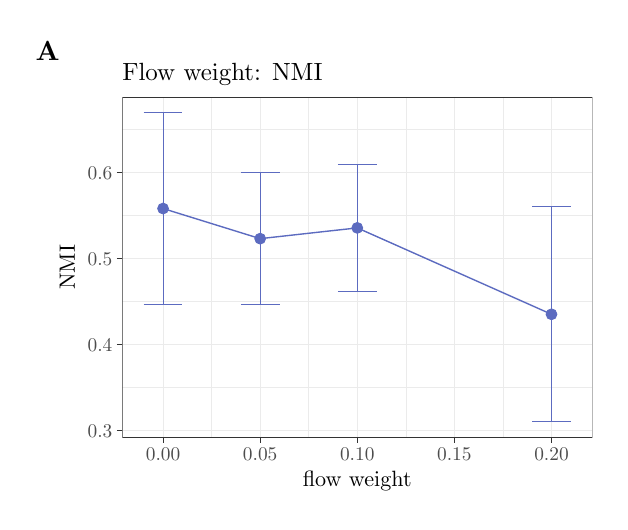
\begin{tikzpicture}[x=1pt,y=1pt]
\definecolor{fillColor}{RGB}{255,255,255}
\path[use as bounding box,fill=fillColor,fill opacity=0.00] (0,0) rectangle (206.87,171.36);
\begin{scope}
\path[clip] (  0.85,  1.87) rectangle (206.02,169.49);
\definecolor{drawColor}{RGB}{255,255,255}
\definecolor{fillColor}{RGB}{255,255,255}

\path[draw=drawColor,line width= 0.4pt,line join=round,line cap=round,fill=fillColor] (  0.85,  1.87) rectangle (206.02,169.49);
\end{scope}
\begin{scope}
\path[clip] ( 34.19, 23.34) rectangle (204.02,146.20);
\definecolor{fillColor}{RGB}{255,255,255}

\path[fill=fillColor] ( 34.19, 23.34) rectangle (204.02,146.20);
\definecolor{drawColor}{gray}{0.92}

\path[draw=drawColor,line width= 0.2pt,line join=round] ( 34.19, 41.31) --
	(204.02, 41.31);

\path[draw=drawColor,line width= 0.2pt,line join=round] ( 34.19, 72.42) --
	(204.02, 72.42);

\path[draw=drawColor,line width= 0.2pt,line join=round] ( 34.19,103.53) --
	(204.02,103.53);

\path[draw=drawColor,line width= 0.2pt,line join=round] ( 34.19,134.64) --
	(204.02,134.64);

\path[draw=drawColor,line width= 0.2pt,line join=round] ( 66.47, 23.34) --
	( 66.47,146.20);

\path[draw=drawColor,line width= 0.2pt,line join=round] (101.56, 23.34) --
	(101.56,146.20);

\path[draw=drawColor,line width= 0.2pt,line join=round] (136.65, 23.34) --
	(136.65,146.20);

\path[draw=drawColor,line width= 0.2pt,line join=round] (171.74, 23.34) --
	(171.74,146.20);

\path[draw=drawColor,line width= 0.4pt,line join=round] ( 34.19, 25.75) --
	(204.02, 25.75);

\path[draw=drawColor,line width= 0.4pt,line join=round] ( 34.19, 56.86) --
	(204.02, 56.86);

\path[draw=drawColor,line width= 0.4pt,line join=round] ( 34.19, 87.97) --
	(204.02, 87.97);

\path[draw=drawColor,line width= 0.4pt,line join=round] ( 34.19,119.08) --
	(204.02,119.08);

\path[draw=drawColor,line width= 0.4pt,line join=round] ( 48.92, 23.34) --
	( 48.92,146.20);

\path[draw=drawColor,line width= 0.4pt,line join=round] ( 84.01, 23.34) --
	( 84.01,146.20);

\path[draw=drawColor,line width= 0.4pt,line join=round] (119.10, 23.34) --
	(119.10,146.20);

\path[draw=drawColor,line width= 0.4pt,line join=round] (154.19, 23.34) --
	(154.19,146.20);

\path[draw=drawColor,line width= 0.4pt,line join=round] (189.28, 23.34) --
	(189.28,146.20);
\definecolor{drawColor}{RGB}{92,107,192}

\path[draw=drawColor,line width= 0.5pt,line join=round] ( 48.92,106.01) --
	( 84.01, 95.12) --
	(119.10, 99.01) --
	(189.28, 67.79);
\definecolor{fillColor}{RGB}{92,107,192}

\path[draw=drawColor,line width= 0.3pt,line join=round,line cap=round,fill=fillColor] ( 48.92,106.01) circle (  1.97);

\path[draw=drawColor,line width= 0.3pt,line join=round,line cap=round,fill=fillColor] ( 84.01, 95.12) circle (  1.97);

\path[draw=drawColor,line width= 0.3pt,line join=round,line cap=round,fill=fillColor] (119.10, 99.01) circle (  1.97);

\path[draw=drawColor,line width= 0.3pt,line join=round,line cap=round,fill=fillColor] (189.28, 67.79) circle (  1.97);

\path[draw=drawColor,line width= 0.3pt,line join=round] ( 41.91,140.61) --
	( 55.94,140.61);

\path[draw=drawColor,line width= 0.3pt,line join=round] ( 48.92,140.61) --
	( 48.92, 71.41);

\path[draw=drawColor,line width= 0.3pt,line join=round] ( 41.91, 71.41) --
	( 55.94, 71.41);

\path[draw=drawColor,line width= 0.3pt,line join=round] ( 77.00,118.95) --
	( 91.03,118.95);

\path[draw=drawColor,line width= 0.3pt,line join=round] ( 84.01,118.95) --
	( 84.01, 71.30);

\path[draw=drawColor,line width= 0.3pt,line join=round] ( 77.00, 71.30) --
	( 91.03, 71.30);

\path[draw=drawColor,line width= 0.3pt,line join=round] (112.09,121.93) --
	(126.12,121.93);

\path[draw=drawColor,line width= 0.3pt,line join=round] (119.10,121.93) --
	(119.10, 76.08);

\path[draw=drawColor,line width= 0.3pt,line join=round] (112.09, 76.08) --
	(126.12, 76.08);

\path[draw=drawColor,line width= 0.3pt,line join=round] (182.26,106.66) --
	(196.30,106.66);

\path[draw=drawColor,line width= 0.3pt,line join=round] (189.28,106.66) --
	(189.28, 28.92);

\path[draw=drawColor,line width= 0.3pt,line join=round] (182.26, 28.92) --
	(196.30, 28.92);
\definecolor{drawColor}{gray}{0.20}

\path[draw=drawColor,line width= 0.4pt,line join=round,line cap=round] ( 34.19, 23.34) rectangle (204.02,146.20);
\end{scope}
\begin{scope}
\path[clip] (  0.00,  0.00) rectangle (206.87,171.36);
\definecolor{drawColor}{gray}{0.30}

\node[text=drawColor,anchor=base east,inner sep=0pt, outer sep=0pt, scale=  0.70] at ( 30.59, 23.34) {0.3};

\node[text=drawColor,anchor=base east,inner sep=0pt, outer sep=0pt, scale=  0.70] at ( 30.59, 54.45) {0.4};

\node[text=drawColor,anchor=base east,inner sep=0pt, outer sep=0pt, scale=  0.70] at ( 30.59, 85.56) {0.5};

\node[text=drawColor,anchor=base east,inner sep=0pt, outer sep=0pt, scale=  0.70] at ( 30.59,116.67) {0.6};
\end{scope}
\begin{scope}
\path[clip] (  0.00,  0.00) rectangle (206.87,171.36);
\definecolor{drawColor}{gray}{0.20}

\path[draw=drawColor,line width= 0.4pt,line join=round] ( 32.19, 25.75) --
	( 34.19, 25.75);

\path[draw=drawColor,line width= 0.4pt,line join=round] ( 32.19, 56.86) --
	( 34.19, 56.86);

\path[draw=drawColor,line width= 0.4pt,line join=round] ( 32.19, 87.97) --
	( 34.19, 87.97);

\path[draw=drawColor,line width= 0.4pt,line join=round] ( 32.19,119.08) --
	( 34.19,119.08);
\end{scope}
\begin{scope}
\path[clip] (  0.00,  0.00) rectangle (206.87,171.36);
\definecolor{drawColor}{gray}{0.20}

\path[draw=drawColor,line width= 0.4pt,line join=round] ( 48.92, 21.34) --
	( 48.92, 23.34);

\path[draw=drawColor,line width= 0.4pt,line join=round] ( 84.01, 21.34) --
	( 84.01, 23.34);

\path[draw=drawColor,line width= 0.4pt,line join=round] (119.10, 21.34) --
	(119.10, 23.34);

\path[draw=drawColor,line width= 0.4pt,line join=round] (154.19, 21.34) --
	(154.19, 23.34);

\path[draw=drawColor,line width= 0.4pt,line join=round] (189.28, 21.34) --
	(189.28, 23.34);
\end{scope}
\begin{scope}
\path[clip] (  0.00,  0.00) rectangle (206.87,171.36);
\definecolor{drawColor}{gray}{0.30}

\node[text=drawColor,anchor=base,inner sep=0pt, outer sep=0pt, scale=  0.70] at ( 48.92, 14.92) {0.00};

\node[text=drawColor,anchor=base,inner sep=0pt, outer sep=0pt, scale=  0.70] at ( 84.01, 14.92) {0.05};

\node[text=drawColor,anchor=base,inner sep=0pt, outer sep=0pt, scale=  0.70] at (119.10, 14.92) {0.10};

\node[text=drawColor,anchor=base,inner sep=0pt, outer sep=0pt, scale=  0.70] at (154.19, 14.92) {0.15};

\node[text=drawColor,anchor=base,inner sep=0pt, outer sep=0pt, scale=  0.70] at (189.28, 14.92) {0.20};
\end{scope}
\begin{scope}
\path[clip] (  0.00,  0.00) rectangle (206.87,171.36);
\definecolor{drawColor}{RGB}{0,0,0}

\node[text=drawColor,anchor=base,inner sep=0pt, outer sep=0pt, scale=  0.80] at (119.10,  5.64) {flow weight};
\end{scope}
\begin{scope}
\path[clip] (  0.00,  0.00) rectangle (206.87,171.36);
\definecolor{drawColor}{RGB}{0,0,0}

\node[text=drawColor,rotate= 90.00,anchor=base,inner sep=0pt, outer sep=0pt, scale=  0.80] at ( 17.05, 84.77) {NMI};
\end{scope}
\begin{scope}
\path[clip] (  0.00,  0.00) rectangle (206.87,171.36);
\definecolor{drawColor}{RGB}{0,0,0}

\node[text=drawColor,anchor=base west,inner sep=0pt, outer sep=0pt, scale=  0.90] at ( 34.19,152.18) {Flow weight: NMI};
\end{scope}
\begin{scope}
\path[clip] (  0.00,  0.00) rectangle (206.87,171.36);
\definecolor{drawColor}{RGB}{0,0,0}

\node[text=drawColor,anchor=base,inner sep=0pt, outer sep=0pt, scale=  1.00] at (  7.20,159.49) {\bfseries A};
\end{scope}
\end{tikzpicture}
